\documentclass[12pt,a4paper,titlepage,oneside]{report}

%%{{{ packages
%% font encoding.
\usepackage[utf8]{inputenc}
\usepackage[T1]{fontenc}
\usepackage{lmodern}
\usepackage{couriers}
%% Customize chapters.
\usepackage{titlesec}
%% bibliography.
\usepackage[backend=bibtex,style=ieee]{biblatex}
%% \includegraphics{name}
\usepackage{graphicx}
%% \url{something}
\usepackage{url}
%% \multirow{package}{width}{text}
\usepackage{multirow}
%% \cellcolor
\usepackage[table]{xcolor}
%% \caption{title}
\usepackage{caption}
\usepackage{subcaption}
%% \forloop
\usepackage{forloop}
%% fix underfull on footnote with URL.
\usepackage{ragged2e}
%% source code listing
\usepackage{listings}
%% \printindex
\usepackage{makeidx}
%% table of content
\usepackage{tocloft}
%% text emphasis, including strikeout.
\usepackage[normalem]{ulem}
%% mathematics
\usepackage{mathtools}
%% arithmetic
\usepackage{calc}
%% algorithm
\usepackage{algorithm}
\usepackage{algpseudocode}
%% multiple columns
\usepackage{multicol}
%% Change the margin
\usepackage[a4paper]{geometry}
\geometry{
	a4paper,
	top=3cm,
	right=3cm,
	bottom=3cm,
	left=4cm
}
%%
\usepackage{parskip}
%% Package for reading CSV to database.
\usepackage{datatool}
%% Package for scatter and line plot.
\usepackage{dataplot}
%% Long table
\usepackage{longtable}
%% Tikz
\usepackage{pgfplots}

%% Add box to figure.
%%
\usepackage{float}

\floatstyle{boxed}
\restylefloat{figure}

%% MnSymbol
\usepackage{MnSymbol}
%%}}}

%%{{{ hyphenation: sorted in ascending.
%%
\hyphenation{
	Ja-nu-a-ri
	SIGKDD
	Wiki-pedia
	a-kan
	ang-ka
	ba-gai-ma-na
	bayes-ian
	ber-kas
	ber-ma-sa-lah
	ber-mak-na
	bi-a-ya
	da-lam
	data-set
	de-ngan
	di-ha-sil-kan
	di-sing-kat
	di-tam-bah-kan
	dis-krit
	fung-si
	ga-bung-an
	ke-las
	ke-mung-ki-nan
	ke-tak-se-imbang-an
	lan-guage
	ma-yo-ri-tas
	me-laku-kan
	me-me-rik-sa
	me-mi-lih
	me-ne-rap-kan
	me-ning-kat-kan
	me-nye-dia-kan
	me-nye-im-bang-kan
	me-sin
	me-thod
	mem-vi-sua-li-sa-si
	meng-gu-na-kan
	meng-hu-bung-kan
	meng-i-kut-kan
	meng-i-kuti
	meng-im-ple-men-ta-si-kan
	meng-in-di-ka-si-kan
	mi-sal-nya
	mung-kin
	o-ver-sam-pling
	pa-ra-lel
	pe-mi-sah
	pe-nan-da
	pe-ne-li-ti-an
	pe-nu-li-san
	pe-nyun-ting
	pem-ban-ding
	pen-de-kat-an
	peng-kla-si-fi-ka-si
	per-for-man-si-nya
	po-ten-si-al
	pro-ba-bi-li-tas
	pro-ses
	sam-pel
	se-im-bang
	se-jum-lah
	sun-ting-an
	ting-kat
	un-der-sam-pling
	wa-lau-pun
}
%%}}}

%%{{{ override default latex setting.
%%

%% Space between paragraphs.
\setlength{\parskip}{1.5em}

%% Add dot to TOC.
\renewcommand{\cftsecleader}{\cftdotfill{\cftdotsep}}
\renewcommand{\contentsname}{}

\lstset{
	basicstyle=\scriptsize\ttfamily
,	breaklines=true
,	stringstyle=\scriptsize\ttfamily
,	numbers=left
,	numberstyle=\tiny\ttfamily
,	numbersep=5pt
,	tabsize=4
,	frame=single
}

\makeatletter
\def\lst@lettertrue{\let\lst@ifletter\iffalse}
\makeatother

%% Format chapter and section.
%%
%%% Set chapter name to Bab.
\titleformat{\chapter}[hang]
{\bfseries\large\centering}
{Bab \thechapter}
{1em}
{}

\titleformat{\section}[hang]
{\bfseries\large}
{\thesection}
{1em}{}

%% Set spacing for sections.
\titlespacing{\chapter}{0ex}{0ex}{1.5em}
\titlespacing{\section}{0ex}{0ex}{0em}

%% Alter latex default title on table.
\captionsetup[table]{name=Tabel}
\captionsetup[figure]{name=Gambar}

\renewcommand{\arraystretch}{1.5}
\setlength{\tabcolsep}{3pt}

%% Change bibliography title.
\defbibheading{bibliography}{\centerline{
	\textbf{DAFTAR REFERENSI}}
}

%%% uncomment this to show overrule in black box
\overfullrule=2cm

%% Algorithmicx
\makeatletter
\renewcommand{\ALG@beginalgorithmic}{\footnotesize}
\makeatother

%% multicolumn setting
\setlength{\columnsep}{1cm}

%% pgfplots setting.
\pgfplotsset{
	/pgf/number format/read comma as period,
	/pgf/text mark as node=false,
	table/col sep=semicolon,
	xmax=1,
	xmin=0,
	ymax=1,
	ymin=0,
	xtick distance=0.2,
	ytick distance=0.2,
	grid=major,
	cycle list name=linestyles,
}
%%}}}

%%{{{ variables
%%
\newcommand{\mytitle}{Deteksi Vandalisme pada Wikipedia Bahasa Inggris menggunakan klasifikasi Cascaded Random Forest}
\newcommand{\myname}{Muhamad Sulhan}
\newcommand{\mysid}{23513014}
\newcommand{\myadvisorname}{Dwi Hendratmo Widyantoro}
\newcommand{\myadvisorid}{196812071994021001}
\newcommand{\mydept}{Program Studi Magister Informatika}
\newcommand{\itb}{Institut Teknologi Bandung}

%%% My images directory
\graphicspath{{../images/}}
\newcommand{\myitbcover}{ITB-logo-hitam}

%%% My bibligraphy file
\addbibresource{bibliography.bib}
%%}}}

%%{{{ document's meta-data
%%
\author{\myname}
\title{\mytitle}
%%}}}

%%{{{ document's macros
%%
%%% two column signature.
\def\myadvisorsig#1{%
	\vbox{\hsize=6cm
		\textbf{#1}\\
		\addvspace{2cm}%
		\hbox to \hsize{%
			\strut\hfil%
			\myadvisorname%
			\hfil%
		}
		\hrule\kern1ex
		\hbox to \hsize{%
			\strut\hfil%
			NIP\hspace{1ex}\myadvisorid%
			\hfil%
		}
	}
}

%%% one column signature.
\def\mysignature#1#2#3{%
	\vbox{
		\textbf{#1}\\
		\addvspace{2cm}%
		\hbox to \hsize{%
			\strut\hfil%
			{#2}%
			\hfil%
		}
		\makebox[6cm][c]{
			\hrulefill
		}
		\hbox to \hsize{%
			\strut\hfil%
			NIP\hspace{1ex}{#3}%
			\hfil%
		}
	}
}

%%% source code listing
\lstdefinelanguage{go}
{
	morekeywords={package,import,const,func,for,type,var,struct}
,	sensitive=true
,	morecomment=[l]{//}
,	morecomment=[s]{/*}{*/}
}
\lstdefinestyle{go}{%
	language=go
,	keywordstyle=\color{black}\bfseries
,	commentstyle=\color{gray}
,	breakatwhitespace=true
,	lineskip={-2.5pt}
}
\newcommand{\includecodego}[2][c]{
	\lstinputlisting[caption=#2,escapechar=,style=go]
		{/home/ms/go/work/src/github.com/shuLhan/#2}
}

%%% data listing
\lstdefinestyle{data}{%
	breakatwhitespace=false
,	breakautoindent=false
,	literate={\,}{}{0\discretionary{,}{}{,}},
}
\newcommand{\includedata}[2][c]{
	\lstinputlisting[caption=#2,style=data,linerange={1-10}]
		{/home/ms/go/work/src/github.com/shuLhan/#2}
}
%%}}}

%%
%% Create cover with parameters
%% 1: report number
%% 2: report weeks, in string
%% 3: report date, string
%%
\newcommand{\reportcover}[3]{
	\thispagestyle{empty}
	\begin{center}\textbf{%
		\mytitle
		\vfill
		Laporan Progres Tesis, Catatan, dan Pekerjaan Selanjutnya
		\linebreak
		Laporan ke-#1
		\linebreak
		Minggu #2
		\linebreak
		\linebreak
		#3
		\vfill
		Oleh \\
		\myname \\
		\mysid \\
		\vfill
		\uppercase{%
			Program Studi Magister Informatika \\
			Sekolah Teknik Elektro dan Informatika \\
			Institut Teknologi Bandung \\
			2015
		}
	}
	\end{center}
	\newpage
}

%%
%% Macro for advisor's signature
%%
\newcommand{\advisorsignature}{
	\vfill
	\begin{center}
		Diketahui oleh,
		\linebreak
		\linebreak
		\hbox to \hsize{%
			\myadvisorsig{Pembimbing,\quad}\hfil
		}
	\end{center}
}

%%
%% Macro for create schedule using parameter
%% 1: number of weeks has passed on task 1
%% 2: number of weeks has passed on task 2
%% 3: number of weeks has passed on task 3
%% 4: number of weeks has passed on task 4
%% 5: should we begin in newpage?
%%

% function to fill cell with color
\newcommand{\tand}{&}
\newcounter{cnt}
\newcommand{\fillcell}[1]{%
	\forloop{cnt}{0}{\value{cnt}<#1}{%
		{\cellcolor[gray]{0.7}} \tand
	}%
}
% function to create empty cell
\newcommand{\emptycell}[2]{%
	\forloop{cnt}{0}{\value{cnt}<#1}{%
		\tand
	}%
	\ifthenelse{#2 = 1}{\\}{\tand}%
}
% function to fill week in progress.
\newcommand{\progresscell}[1]{%
	\forloop{cnt}{0}{\value{cnt}<#1}{%
		{\cellcolor{red!80}} \tand
	}%
}

\newcommand{\schedule}[4]{
	\section{Penjadwalan}\label{sec:penjadwalan}

Tabel di bawah menampilkan jadwal yang direncanakan dalam pengembangan tesis dari bulan ke I, September 2015, sampai dengan bulan ke VI, Januari 2016.

Warna merah menandakan minggu yang telah lewat sampai minggu dari laporan progres ini, untuk warna abu-abu menandakan waktu pelaksanaan yang akan datang.

\newcounter{planone}
\newcounter{plantwo}
\newcounter{planthree}
\newcounter{planfour}

\newcounter{progressone}
\newcounter{progresstwo}
\newcounter{progressthree}
\newcounter{progressfour}

\setcounter{progressone}{#1}
\setcounter{progresstwo}{#2}
\setcounter{progressthree}{#3}
\setcounter{progressfour}{#4}

\setcounter{planone}{4 - \theprogressone}
\setcounter{plantwo}{17 - \theprogresstwo}
\setcounter{planthree}{14 - \theprogressthree}
\setcounter{planfour}{2 - \theprogressfour}

\begin{table}[h!]
	\centering
	{\footnotesize
	\begin{tabular}{|c|p{0.2\textwidth}
	|c|c|c|c
	|c|c|c|c
	|c|c|c|c
	|c|c|c|c
	|c|c|c|c
	|c|c|c|c|}
		\hline
		\multirow{2}{*}{No.}
			& \multirow{2}{*}{Kegiatan}
			& \multicolumn{4}{c|}{Bulan I}
			& \multicolumn{4}{c|}{Bulan II}
			& \multicolumn{4}{c|}{Bulan III}
			& \multicolumn{4}{c|}{Bulan IV}
			& \multicolumn{4}{c|}{Bulan V}
			& \multicolumn{4}{c|}{Bulan VI}\\
		\cline{3-26}
		& &
			1 & 2 & 3 & 4 &
			1 & 2 & 3 & 4 &
			1 & 2 & 3 & 4 &
			1 & 2 & 3 & 4 &
			1 & 2 & 3 & 4 &
			1 & 2 & 3 & 4\\
		\hline
		1 & Persiapan\ \  Data dan\ \ Lingkungan Penelitian &
			\progresscell{\theprogressone}
			\fillcell{\theplanone}
			\emptycell{19}{1}
		\hline
		2 & Implementasi dan Pengujian &
			\emptycell{2}{0}
			\progresscell{\theprogresstwo}
			\fillcell{\theplantwo}
			\emptycell{3}{1}
		\hline
		4 & Analisis &
			\emptycell{7}{0}
			\progresscell{\theprogressthree}
			\fillcell{\theplanthree}
			\emptycell{1}{1}
		\hline
		5 & Evaluasi &
			\emptycell{20}{0}
			\progresscell{\theprogressfour}
			\fillcell{\theplanfour}
			\emptycell{0}{1}
		\hline
	\end{tabular}
	}
	\caption{Jadwal penelitian tesis}
\end{table}
}




%%
%% DOCUMENT
%%
\begin{document}
\reportcover{V}{15 dan 16}{4 Januari 2016}

\section{Pendahuluan}

\subsection{Perbaikan Algoritma CART}

Kesalahan yang dilakukan pada implementasi sebelumnya yaitu pada penggunaan
atribut untuk pemisahan \textit{tree}.
Jika sebuah atribut telah digunakan sebagai pemisah, dan menjadi sebuah
\textit{node} pada pohon keputusan, maka atribut tersebut tidak boleh diproses
atau menjadi pemisah kembali pada anak-anaknya, namun bisa diproses kembali
pada \textit{grandchild}-nya.

Hal seperti ini tidak pernah disebutkan dalam teks algoritma CART,
sehingga saya cukup kesulitan menemukan kesalahan yang dilakukan.

\subsection{Implementasi Random Forest}

Implemetansi algoritma \textit{ensemble} \textit{Random Forest} (RF) secara
umum mengacu pada buku Friedman, dkk. \cite{friedman2001elements}, dengan
tambahan dari video kuliah dan tulisan lain di internet.

Algoritma RF yang diimplementasikan menggunakan teknik \textit{bagging},
\textit{out-of-bag} (OOB), dan CART sebagai pengklasifikasi di setiap pohon
keputusan.

\clearpage

Berikut algoritma RF yang digunakan,

\begin{lstlisting}
FUNGSI RandomForest
INPUT
	D: dataset
	NTREE: jumlah tree
	NFEATURE: jumlah fitur yang dipilih secara acak
	NBAGGING: jumlah sub-sampel yang dipilih secara acak dengan
	replacement, dalam nilai persentase.
OUTPUT
	FOREST: kumpulan tree
VAR
	SUMOOBERROR: total galat untuk OOB
BEGIN
	SUMOOBERROR := 0.0

	FOR i = 0; i < NTREE; i++
	BEGIN
		subsample, oob := RandomPickRows(D, NBAGGING)

		subfeature := RandomPickColumns(subsample, NFEATURE)

		cartTree := CreateTree(subfeature)

		ooberror := cartTree.CountOOBError(oob)

		SUMOOBERROR += ooberror

		FOREST.AddTree(cartTree)
	END

	FOREST.AverageOOBError = SUMOOBERROR / NTREE
END
\end{lstlisting}

Hasil implementasi kemudian diuji dengan dataset \textit{Glass Identification}
\cite{evett1987rule}, dengan jumlah sample yaitu 124, jumlah fitur 9, jumlah
kelas yaitu 7 (contoh data bisa dilihat pada lampiran
\ref{appendix:dataset_glass}),
Hasilnya dalam bentuk grafik penghitungan laju galat OOB yang dapat dilihat
pada gambar \ref{fig:rf_glass}.

\begin{figure}[t]
	\centering
	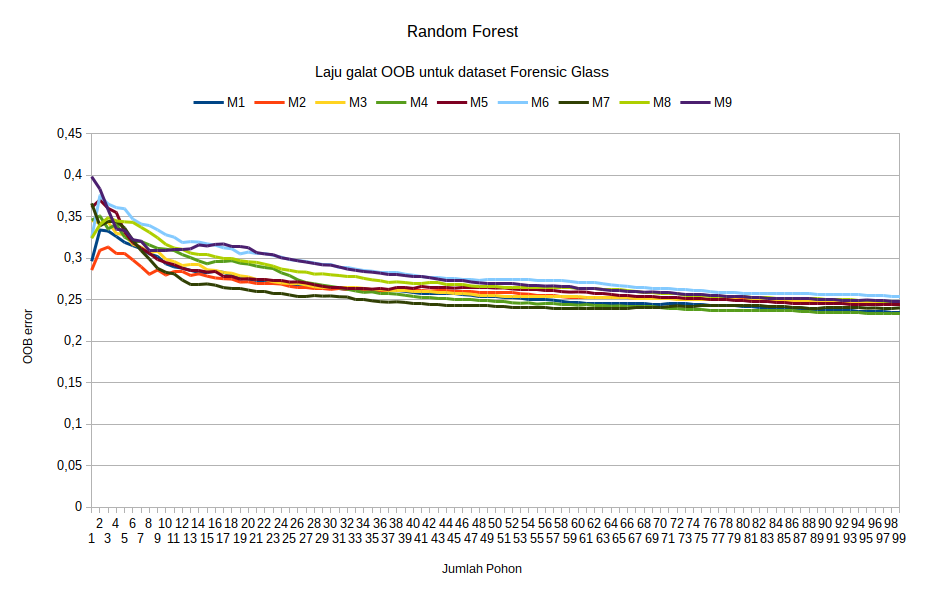
\includegraphics[keepaspectratio=true,scale=0.5]{rf_glass}
	\caption{OOB laju error pada Random Forest untuk dataset Forensic Glass
	dengan jumlah fitur secara acak dari 2 sampai 9.}
	\label{fig:rf_glass}
\end{figure}

Dataset diuji dengan mengambil dua per tiga (66\%) dari data asli untuk
\textit{bootstrap} dan sisanya digunakan sebagai latihan (OOB) untuk
mendapatkan galat, dengan jumlah tree yang digunakan yaitu 50.


\section{Laporan Singkat Progres}

Pekerjaan yang telah dilakukan,
\begin{itemize}
\item perbaikan algoritma CART
\item implementasi algoritma \textit{Random Forest}
\end{itemize}
%%}}}

\section{Catatan}

\subsection{Perbaikan Algoritma CART}

Kesalahan yang dilakukan pada implementasi sebelumnya yaitu pada penggunaan
atribut untuk pemisahan \textit{tree}.
Jika sebuah atribut telah digunakan sebagai pemisah, dan menjadi sebuah
\textit{node} pada pohon keputusan, maka atribut tersebut tidak boleh diproses
atau menjadi pemisah kembali pada anak-anaknya, namun bisa diproses kembali
pada \textit{grandchild}-nya.

Hal seperti ini tidak pernah disebutkan dalam teks algoritma CART,
sehingga saya cukup kesulitan menemukan kesalahan yang dilakukan.

\subsection{Implementasi Random Forest}

Implemetansi algoritma \textit{ensemble} \textit{Random Forest} (RF) secara
umum mengacu pada buku Friedman, dkk. \cite{friedman2001elements}, dengan
tambahan dari video kuliah dan tulisan lain di internet.

Algoritma RF yang diimplementasikan menggunakan teknik \textit{bagging},
\textit{out-of-bag} (OOB), dan CART sebagai pengklasifikasi di setiap pohon
keputusan.

\clearpage

Berikut algoritma RF yang digunakan,

\begin{lstlisting}
FUNGSI RandomForest
INPUT
	D: dataset
	NTREE: jumlah tree
	NFEATURE: jumlah fitur yang dipilih secara acak
	NBAGGING: jumlah sub-sampel yang dipilih secara acak dengan
	replacement, dalam nilai persentase.
OUTPUT
	FOREST: kumpulan tree
VAR
	SUMOOBERROR: total galat untuk OOB
BEGIN
	SUMOOBERROR := 0.0

	FOR i = 0; i < NTREE; i++
	BEGIN
		subsample, oob := RandomPickRows(D, NBAGGING)

		subfeature := RandomPickColumns(subsample, NFEATURE)

		cartTree := CreateTree(subfeature)

		ooberror := cartTree.CountOOBError(oob)

		SUMOOBERROR += ooberror

		FOREST.AddTree(cartTree)
	END

	FOREST.AverageOOBError = SUMOOBERROR / NTREE
END
\end{lstlisting}

Hasil implementasi kemudian diuji dengan dataset \textit{Glass Identification}
\cite{evett1987rule}, dengan jumlah sample yaitu 124, jumlah fitur 9, jumlah
kelas yaitu 7 (contoh data bisa dilihat pada lampiran
\ref{appendix:dataset_glass}),
Hasilnya dalam bentuk grafik penghitungan laju galat OOB yang dapat dilihat
pada gambar \ref{fig:rf_glass}.

\begin{figure}[t]
	\centering
	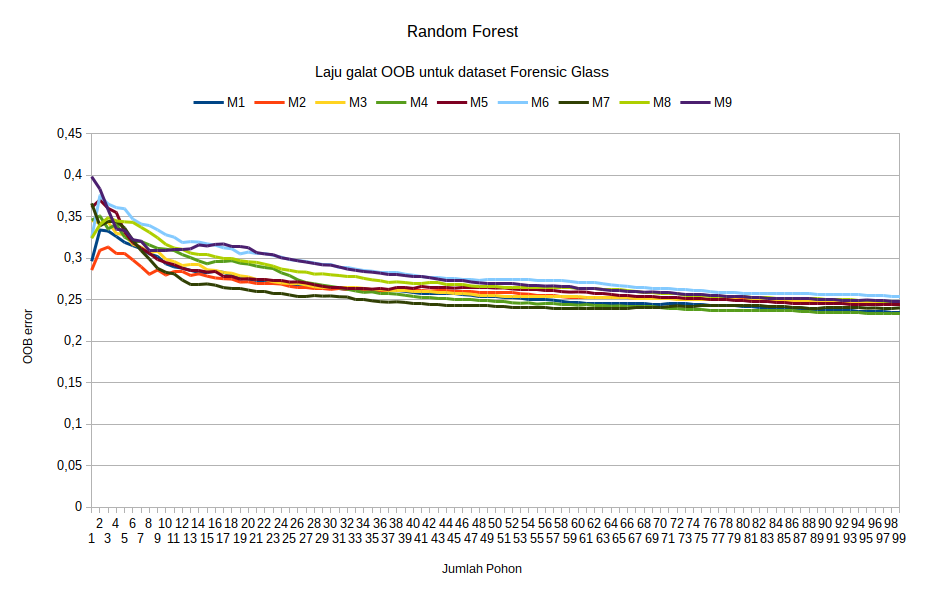
\includegraphics[keepaspectratio=true,scale=0.5]{rf_glass}
	\caption{OOB laju error pada Random Forest untuk dataset Forensic Glass
	dengan jumlah fitur secara acak dari 2 sampai 9.}
	\label{fig:rf_glass}
\end{figure}

Dataset diuji dengan mengambil dua per tiga (66\%) dari data asli untuk
\textit{bootstrap} dan sisanya digunakan sebagai latihan (OOB) untuk
mendapatkan galat, dengan jumlah tree yang digunakan yaitu 50.


\clearpage
\section{Pekerjaan Selanjutnya}

Berikut garis besar tahap yang akan dikerjakan untuk pekerjaan selanjutnya,

\begin{itemize}
\item Mempelajari dan mengimplementasikan \textit{Cascaded Random Forest}.
\item Implementasi algoritma LN-SMOTE.
\item Mempelajari tentang kurva ROC and AUC.
\item Implementasi penghitungan fitur.
\item Menerapkan algoritma SMOTE dan LN-SMOTE pada hasil penghitungan fitur.
\item Menerapkan \textit{Random Forest} pada hasil \textit{resampling} SMOTE
dan LN-SMOTE.
\item Menerapkan algoritma \textit{Cascade Random Forest} dari hasil SMOTE dan
LN-SMOTE.
\item Membandingkan hasil dari klasifikasi \textit{Random Forest} dan
\textit{Cascaded RandomForest}
\end{itemize}

\clearpage
\schedule{4}{13}{0}{0}

\advisorsignature

\clearpage
\addcontentsline{toc}{section}{Daftar Referensi}
\printbibliography

\newpage
\appendix
\subsection{Perbaikan Algoritma CART}

Kesalahan yang dilakukan pada implementasi sebelumnya yaitu pada penggunaan
atribut untuk pemisahan \textit{tree}.
Jika sebuah atribut telah digunakan sebagai pemisah, dan menjadi sebuah
\textit{node} pada pohon keputusan, maka atribut tersebut tidak boleh diproses
atau menjadi pemisah kembali pada anak-anaknya, namun bisa diproses kembali
pada \textit{grandchild}-nya.

Hal seperti ini tidak pernah disebutkan dalam teks algoritma CART,
sehingga saya cukup kesulitan menemukan kesalahan yang dilakukan.

\subsection{Implementasi Random Forest}

Implemetansi algoritma \textit{ensemble} \textit{Random Forest} (RF) secara
umum mengacu pada buku Friedman, dkk. \cite{friedman2001elements}, dengan
tambahan dari video kuliah dan tulisan lain di internet.

Algoritma RF yang diimplementasikan menggunakan teknik \textit{bagging},
\textit{out-of-bag} (OOB), dan CART sebagai pengklasifikasi di setiap pohon
keputusan.

\clearpage

Berikut algoritma RF yang digunakan,

\begin{lstlisting}
FUNGSI RandomForest
INPUT
	D: dataset
	NTREE: jumlah tree
	NFEATURE: jumlah fitur yang dipilih secara acak
	NBAGGING: jumlah sub-sampel yang dipilih secara acak dengan
	replacement, dalam nilai persentase.
OUTPUT
	FOREST: kumpulan tree
VAR
	SUMOOBERROR: total galat untuk OOB
BEGIN
	SUMOOBERROR := 0.0

	FOR i = 0; i < NTREE; i++
	BEGIN
		subsample, oob := RandomPickRows(D, NBAGGING)

		subfeature := RandomPickColumns(subsample, NFEATURE)

		cartTree := CreateTree(subfeature)

		ooberror := cartTree.CountOOBError(oob)

		SUMOOBERROR += ooberror

		FOREST.AddTree(cartTree)
	END

	FOREST.AverageOOBError = SUMOOBERROR / NTREE
END
\end{lstlisting}

Hasil implementasi kemudian diuji dengan dataset \textit{Glass Identification}
\cite{evett1987rule}, dengan jumlah sample yaitu 124, jumlah fitur 9, jumlah
kelas yaitu 7 (contoh data bisa dilihat pada lampiran
\ref{appendix:dataset_glass}),
Hasilnya dalam bentuk grafik penghitungan laju galat OOB yang dapat dilihat
pada gambar \ref{fig:rf_glass}.

\begin{figure}[t]
	\centering
	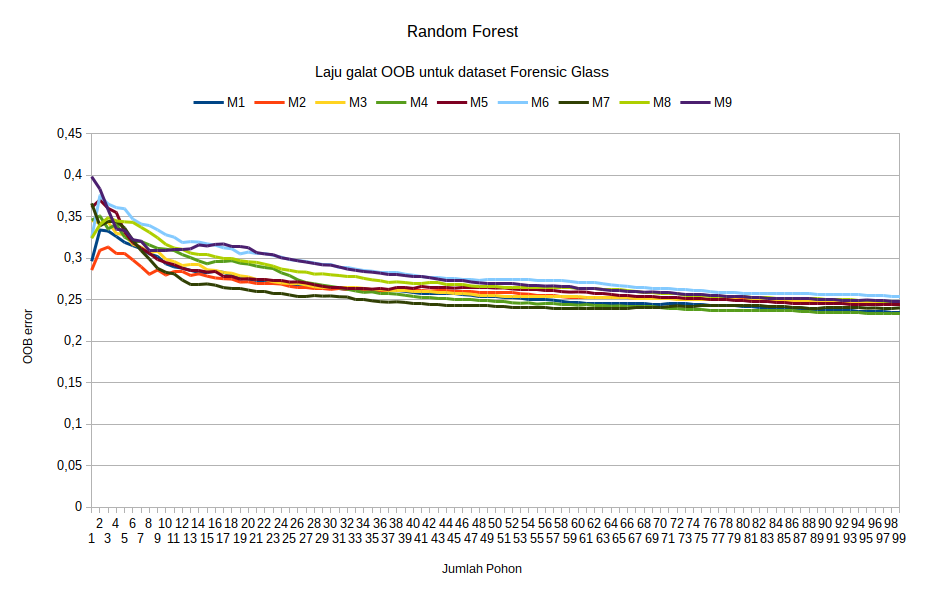
\includegraphics[keepaspectratio=true,scale=0.5]{rf_glass}
	\caption{OOB laju error pada Random Forest untuk dataset Forensic Glass
	dengan jumlah fitur secara acak dari 2 sampai 9.}
	\label{fig:rf_glass}
\end{figure}

Dataset diuji dengan mengambil dua per tiga (66\%) dari data asli untuk
\textit{bootstrap} dan sisanya digunakan sebagai latihan (OOB) untuk
mendapatkan galat, dengan jumlah tree yang digunakan yaitu 50.


\end{document}
